\documentclass[11pt]{article}
\usepackage[margin=1in]{geometry}
\usepackage{amsmath,amssymb,amsthm}
\usepackage{bm}
\usepackage{graphicx}
\usepackage{subcaption}
\usepackage{booktabs}
\usepackage{longtable}
\usepackage{array}
\usepackage{float}
\usepackage{xcolor}
\usepackage{listings}
\usepackage{tikz}
\usepackage[T1]{fontenc}
\usepackage[utf8]{inputenc}
\usepackage{lmodern}
\usepackage{microtype}
\usepackage{hyperref}

\usetikzlibrary{arrows.meta,positioning}
\hypersetup{colorlinks=true,linkcolor=blue,citecolor=blue,urlcolor=blue}

\lstset{
  basicstyle=\ttfamily\small,
  breaklines=true,
  columns=fullflexible,
  frame=single,
  rulecolor=\color{black!30}
}

\title{Single-Surface Finite-Beta Boozer Optimization in \texttt{simsopt}\\Model, Derivation, Algorithms, Diagnostics, and Current Results}
\author{Generated for the local \texttt{simsopt} checkout}
\date{\today}

\begin{document}
\maketitle

\begin{abstract}
This report documents the finite-beta Boozer-surface workflow implemented in the local \texttt{simsopt} checkout centered on \texttt{examples/2\_Intermediate/boozerQA\_finitebeta.py}. The guiding objective is narrow and specific: retain the direct Boozer-surface philosophy of the vacuum methods of Giuliani et al. \cite{Giuliani2022,Giuliani2023}, but extend it to a finite-pressure setting without embedding VMEC or another full-volume equilibrium solve inside each inner optimization step. The implemented closure is a self-consistent single-surface model in which the total surface field is built from the Boozer tangent representation, the exterior field is extracted from that same surface field by a direct virtual-casing operator, and the resulting exterior field is matched to the coil Biot--Savart field while pressure balance is enforced on the same discretized surface.

The code now contains five core additions: a direct \texttt{VirtualCasing.from\_surface(...)} path, finite-beta surface-field and residual builders, an inner nonlinear least-squares solve in \texttt{FiniteBetaBoozerSurface}, a hybrid Jacobian path that combines exact scalar derivatives with structured finite differences for free-surface geometry, and report-quality diagnostics including surface maps, objective histories, pressure scans, and geometry comparison figures. A new frozen-state comparison also evaluates the direct principal-value closure and the full virtual-casing operator on identical saved states. On the reduced final direct state at nominal $1\%$ beta, the exterior field differs by only $4.61 \times 10^{-3}$ in relative norm, while the replayed pressure and sheet-current blocks remain much farther apart. The present method goes beyond vacuum direct Boozer optimization by introducing a finite-beta surface closure that does not require repeated volume equilibria, but it does not claim to replace full free-boundary MHD equilibrium solvers. It should be interpreted as a tractable optimization model on one surface, not as a proof of the existence of a globally nested finite-beta equilibrium.
\end{abstract}

\tableofcontents
\newpage

\section{Introduction and Literature Context}
Direct optimization of stellarator coils and magnetic surfaces in Boozer coordinates has recently become practical in vacuum by solving for the surface directly instead of repeatedly tracing field lines and post-processing the result \cite{Giuliani2022,Giuliani2023,Wechsung2022}. That direct Boozer framework is attractive because it yields a clean inner optimization problem on one surface, with a geometry-dependent residual that can be embedded in outer coil or surface optimization. The vacuum setting is structurally favorable because the magnetic field is known everywhere once the coils are known.

Finite pressure changes that picture. In a finite-beta equilibrium the field is no longer determined solely by the exterior coils, because plasma current and pressure-induced force balance modify the magnetic stress. Classical stellarator finite-beta optimization therefore relies on equilibrium solvers such as VMEC or related full-volume MHD models \cite{HirshmanWhitson1983,Baillod2022}. Those approaches are indispensable for global equilibrium validation, but they are too expensive and too intrusive to place blindly inside every inner direct-Boozer iteration if the goal is to preserve the lightweight architecture of the vacuum \texttt{boozerQA.py} workflow.

The gap addressed here is therefore the following.

\begin{quote}
Can one construct a useful finite-beta analogue of the direct Boozer inner solve that remains a single-surface problem, uses only surgical changes to \texttt{simsopt}, and avoids a nested VMEC solve in the loop?
\end{quote}

The answer implemented in this checkout is yes, with an important qualification. The method is a \emph{surface closure model}. It enforces the finite-beta jump conditions, tangency, and coil matching on one candidate surface, using the virtual-casing principle to separate the exterior field from the total field directly on that surface. This gives a self-consistent finite-beta optimization model that is much closer to the direct Boozer philosophy than a full equilibrium solve, but it does not by itself guarantee the existence of a globally nested 3D equilibrium.

The finite-beta workflow described here builds on the following established threads:

\begin{itemize}
\item Boozer-coordinate equilibrium theory and surface-field representations \cite{Boozer1981}.
\item Direct Boozer-surface and coil optimization in vacuum \cite{Giuliani2022,Giuliani2023,Wechsung2022}.
\item SIMSOPT as the software framework hosting those optimization loops \cite{Landreman2021}.
\item Finite-beta stellarator optimization based on full equilibrium calculations \cite{Baillod2022}.
\item High-order virtual-casing quadrature used to split internal and external magnetic fields on a surface \cite{Malhotra2020}.
\end{itemize}

Relative to the literature, the central contribution of this implementation is not a new equilibrium theorem. It is an algorithmic and software contribution: a direct finite-beta single-surface closure that can be optimized inside \texttt{simsopt} without handing control of every inner iteration to VMEC.

\section{Scientific Goal and Problem Statement}
The target problem is to construct a surface that is simultaneously:

\begin{enumerate}
\item compatible with a Boozer-surface tangent-field representation,
\item consistent with the magnetic pressure jump associated with a prescribed pressure difference,
\item matched to the exterior field generated by the coils,
\item and sufficiently close to quasisymmetry to serve as the inner target of an outer optimization.
\end{enumerate}

The workflow is intentionally built around a single surface rather than a full volume. This makes the method suitable for design iteration, fast diagnostics, and reduced outer optimization, while preserving a clear path to later validation against full finite-beta equilibria.

\subsection{What is and is not being claimed}
The current code \emph{does} compute a finite-beta Boozer surface using a self-consistent closure on one surface. It \emph{does not} claim to eliminate virtual casing from the mathematics. On the contrary, virtual casing is the central operator used to identify the exterior field associated with the current surface field. The accurate claim is the following:

\begin{quote}
The implementation avoids repeated full-volume equilibrium solves and avoids requiring an auxiliary VMEC-generated virtual-casing input file for the primary inner loop, because the virtual-casing operator is now built directly from the current surface geometry and the current surface field.
\end{quote}

This distinction matters. The method is ``no VMEC in the loop,'' not ``no virtual casing in the loop.''

\section{Single-Surface Finite-Beta Model}
\subsection{Surface geometry and Boozer tangent field}
Let the candidate surface be parameterized by toroidal and poloidal angles $(\varphi,\theta)$:
\begin{equation}
  \mathbf{x} = \mathbf{x}(\varphi,\theta).
\end{equation}
Define the tangent vectors and oriented area element
\begin{equation}
  \mathbf{x}_{\varphi} = \frac{\partial \mathbf{x}}{\partial \varphi},
  \qquad
  \mathbf{x}_{\theta} = \frac{\partial \mathbf{x}}{\partial \theta},
  \qquad
  \mathbf{N} = \mathbf{x}_{\varphi} \times \mathbf{x}_{\theta},
  \qquad
  \hat{\mathbf{n}} = \frac{\mathbf{N}}{|\mathbf{N}|}.
\end{equation}

Following the same direct-Boozer philosophy as the vacuum problem, define the Boozer tangent vector
\begin{equation}
  \mathbf{t} = \mathbf{x}_{\varphi} + \iota \, \mathbf{x}_{\theta}.
\end{equation}
The surface field used in the finite-beta model is then
\begin{equation}
  \mathbf{B}_{\mathrm{total}} = \frac{\Lambda}{|\mathbf{t}|^2} \, \mathbf{t},
  \label{eq:Btotal}
\end{equation}
with
\begin{equation}
  \Lambda = G + \iota I.
\end{equation}
Here $G$ is the Boozer current term associated with the net exterior coil current linkage, and $I$ is the effective poloidal-current scalar associated with the plasma response. The surface-only problem does not determine $G$ and $I$ independently; it determines the combination $\Lambda$ appearing in \eqref{eq:Btotal}. Once $G$ is fixed from the coil currents, the implied current term is recovered by
\begin{equation}
  I = \frac{\Lambda - G}{\iota},
  \qquad \iota \neq 0.
\end{equation}

This is one of the important conceptual corrections made during the implementation. The natural scalar unknown of the inner finite-beta surface problem is $\Lambda$, not $I$ by itself.

\subsection{Virtual-casing closure on the same surface}
The exterior field is computed by the virtual-casing operator from the same total surface field and the same surface geometry:
\begin{equation}
  \mathbf{B}_{\mathrm{external}} = \mathcal{V}[\mathbf{x}, \mathbf{B}_{\mathrm{total}}].
  \label{eq:VCoperator}
\end{equation}
In the compiled library wrapped by \texttt{simsopt}, $\mathcal{V}$ is a high-order singular-quadrature field-transfer operator \cite{Malhotra2020}. The key software advance in this branch is that the wrapper now accepts an arbitrary \texttt{simsopt} surface and arbitrary sampled surface field through \texttt{VirtualCasing.from\_surface(...)}, rather than only a VMEC equilibrium.

The coil field is the Biot--Savart field evaluated on the same surface:
\begin{equation}
  \mathbf{B}_{\mathrm{coils}} = \mathbf{B}_{\mathrm{BS}}[\text{coils}](\mathbf{x}(\varphi,\theta)).
\end{equation}

\subsection{Finite-beta residual equations}
The single-surface finite-beta closure enforces three physics blocks on each quadrature node:

\paragraph{Exterior coil matching}
\begin{equation}
  \mathbf{r}_{\mathrm{coil}} = \mathbf{B}_{\mathrm{external}} - \mathbf{B}_{\mathrm{coils}}.
  \label{eq:rcoil}
\end{equation}

\paragraph{Exterior tangency}
\begin{equation}
  r_{\mathrm{normal}} = \mathbf{B}_{\mathrm{external}} \cdot \hat{\mathbf{n}}.
  \label{eq:rnormal}
\end{equation}

\paragraph{Magnetic pressure balance}
\begin{equation}
  r_{\mathrm{pressure}} = |\mathbf{B}_{\mathrm{external}}|^2 - |\mathbf{B}_{\mathrm{total}}|^2 - 2\mu_0 \Delta p.
  \label{eq:rpressure}
\end{equation}

The diagnostic surface current implied by the field jump is
\begin{equation}
  \mathbf{K} = \frac{\hat{\mathbf{n}} \times \left(\mathbf{B}_{\mathrm{external}} - \mathbf{B}_{\mathrm{total}}\right)}{\mu_0}.
  \label{eq:sheetcurrent}
\end{equation}
This quantity is reported and plotted, but it is not yet promoted to an independent current-potential solve in the primary VC-closed workflow.

\subsection{Residual size and degrees of freedom}
If the surface has $N_c$ active geometric coefficients and the surface grid has $N = n_{\phi} n_{\theta}$ nodes, then the free-surface inner unknown vector is
\begin{equation}
  \mathbf{u} = (c_1,\dots,c_{N_c},\iota,\Lambda) \in \mathbb{R}^{N_c+2}.
\end{equation}
The pointwise residual contributes $3N$ coil-matching equations, $N$ tangency equations, and $N$ pressure-balance equations. When the surface is allowed to move, the code also appends scalar constraints that pin the surface label and anchor the parameterization. The resulting least-squares problem is therefore strongly overdetermined. That is deliberate and mirrors the numerical structure of the vacuum direct Boozer problem \cite{Giuliani2022,Giuliani2023}.

\section{Derivatives and Nonlinear Algorithm}
\subsection{Least-squares solve and block scaling}
The nonlinear inner problem is solved by \texttt{scipy.optimize.least\_squares}. The implementation does not simply concatenate \eqref{eq:rcoil}--\eqref{eq:rpressure} with unit weights, because the blocks live on different numerical scales. Instead the code computes adaptive scaling factors from the coil field strength, the target pressure jump, and the current residual magnitudes, then solves a weighted least-squares problem of the form
\begin{equation}
  \min_{\mathbf{u}} \, \left\| W_{\mathrm{coil}} \mathbf{r}_{\mathrm{coil}} \right\|_2^2 + \left\| W_{\mathrm{normal}} r_{\mathrm{normal}} \right\|_2^2 + \left\| W_{\mathrm{pressure}} r_{\mathrm{pressure}} \right\|_2^2 + \left\| W_{\mathrm{geom}} r_{\mathrm{geom}} \right\|_2^2.
\end{equation}
This weighted form is what made the finite-beta closure numerically usable in practice. Without it, the pressure block can be under-weighted relative to coil matching or vice versa, depending on the surface and pressure scale.

\subsection{Exact fixed-surface derivatives with respect to \texorpdfstring{$\iota$ and $\Lambda$}{iota and Lambda}}
For fixed geometry, the field \eqref{eq:Btotal} can be differentiated analytically. Writing $\mathbf{t}=\mathbf{x}_{\varphi}+\iota \mathbf{x}_{\theta}$, one obtains
\begin{equation}
  \frac{\partial \mathbf{B}_{\mathrm{total}}}{\partial \Lambda} = \frac{\mathbf{t}}{|\mathbf{t}|^2},
\end{equation}
and
\begin{equation}
  \frac{\partial \mathbf{B}_{\mathrm{total}}}{\partial \iota} =
  \Lambda\left(
    \frac{\mathbf{x}_{\theta}}{|\mathbf{t}|^2}
    - 2 \, \frac{\mathbf{t} (\mathbf{t} \cdot \mathbf{x}_{\theta})}{|\mathbf{t}|^4}
  \right).
\end{equation}
For fixed geometry the virtual-casing operator is linear in the input field, so
\begin{equation}
  \frac{\partial \mathbf{B}_{\mathrm{external}}}{\partial \alpha}
  = \mathcal{V}\left[\frac{\partial \mathbf{B}_{\mathrm{total}}}{\partial \alpha}\right],
  \qquad \alpha \in \{\iota,\Lambda\}.
\end{equation}
These exact columns are implemented in \texttt{single\_surface\_vc\_parameter\_jacobian(...)} and validated against finite differences in the test suite.

\subsection{Why a hybrid free-surface Jacobian was needed}
The harder problem is differentiation with respect to surface geometry. The compiled virtual-casing operator in this environment exposes repeated application to a fixed configured operator and exposes field-gradient outputs, but it does not expose an exact source-surface shape derivative of the operator itself. Therefore a fully analytic free-surface Jacobian for the entire VC-closed residual is not currently available without deeper library changes.

The implemented compromise is a hybrid Jacobian:
\begin{equation}
  J = \left[ J_{\mathrm{surf}}^{\mathrm{FD}} \;\middle|\; J_{\iota}^{\mathrm{exact}} \;\middle|\; J_{\Lambda}^{\mathrm{exact}} \right].
\end{equation}
Here the scalar columns are exact, while the surface block is built by structured forward differences using the current residual evaluation cache. This is materially better than a raw black-box \texttt{jac='2-point'} call on all variables, because it preserves the exact scalar physics sensitivities and reuses the expensive baseline VC evaluation consistently.

\subsection{Pressure continuation}
Nonzero pressure jumps are activated through continuation. Rather than jumping directly to the target $\Delta p$, the solver walks through a schedule
\begin{equation}
  0 = \Delta p_0 < \Delta p_1 < \cdots < \Delta p_M = \Delta p_{\mathrm{target}},
\end{equation}
using the solution at one stage as the initial guess for the next. This continuation path is recorded in the solve history together with weighted residual norms, raw residual norms, coil-match norms, normal norms, and pressure norms.

\subsection{Outer loop and pressure scan}
The example also supports a reduced outer quasi-axisymmetry loop and a pressure scan. The outer loop intentionally touches only a reduced set of coil degrees of freedom so that the finite-beta workflow remains practical for development. The pressure scan walks from the vacuum limit to the target pressure jump and reports how $\iota$, $\Lambda$, major radius, and the non-quasisymmetric ratio evolve with pressure.

\section{Algorithmic Workflow}
Figure \ref{fig:workflow} summarizes the implemented workflow.

\begin{figure}[H]
\centering
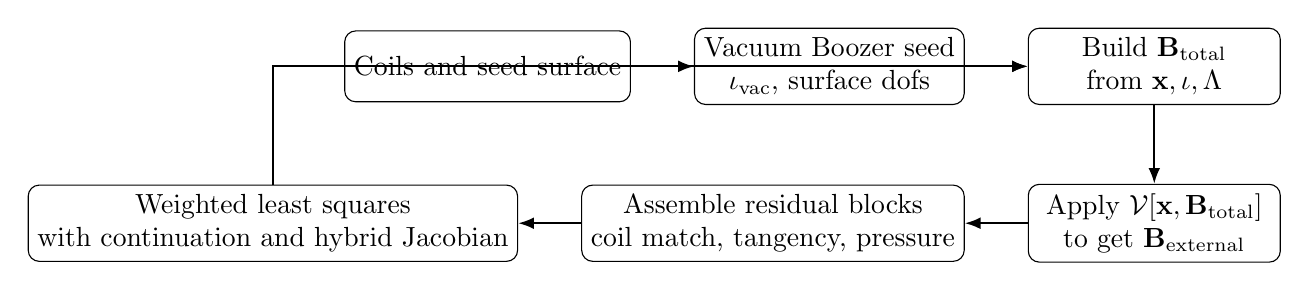
\begin{tikzpicture}[
  node distance=10mm and 8mm,
  box/.style={draw, rounded corners, align=center, minimum width=32mm, minimum height=9mm},
  arr/.style={-{Latex[length=2mm]}, thick}
]
\node[box] (coils) {Coils and seed surface};
\node[box, right=of coils] (vacuum) {Vacuum Boozer seed\\$\iota_{\mathrm{vac}}$, surface dofs};
\node[box, right=of vacuum] (field) {Build $\mathbf{B}_{\mathrm{total}}$\\from $\mathbf{x},\iota,\Lambda$};
\node[box, below=of field] (vc) {Apply $\mathcal{V}[\mathbf{x},\mathbf{B}_{\mathrm{total}}]$\\to get $\mathbf{B}_{\mathrm{external}}$};
\node[box, left=of vc] (res) {Assemble residual blocks\\coil match, tangency, pressure};
\node[box, left=of res] (solve) {Weighted least squares\\with continuation and hybrid Jacobian};

\draw[arr] (coils) -- (vacuum);
\draw[arr] (vacuum) -- (field);
\draw[arr] (field) -- (vc);
\draw[arr] (vc) -- (res);
\draw[arr] (res) -- (solve);
\draw[arr] (solve) |- (field);
\end{tikzpicture}
\caption{Implemented inner finite-beta workflow. The outer coil QA loop wraps around the weighted least-squares solve, but the essential new physics closure is the single-surface map $\mathbf{B}_{\mathrm{total}} \mapsto \mathbf{B}_{\mathrm{external}}$ through virtual casing on the current surface.}
\label{fig:workflow}
\end{figure}

\section{Mapping the Mathematics to the Code}
The implementation is concentrated in a small number of files and intentionally leaves the vacuum path intact.

\begin{longtable}{>{\raggedright\arraybackslash}p{0.30\linewidth} >{\raggedright\arraybackslash}p{0.62\linewidth}}
\toprule
File or function & Role in the finite-beta workflow \\
\midrule
\endhead
\texttt{src/simsopt/mhd/virtual\_casing.py} & Adds \texttt{VirtualCasing.from\_surface(...)} so the VC operator can be built directly from an arbitrary \texttt{simsopt} surface and a sampled surface field. This removes the old dependence on VMEC-produced surface data for the primary inner loop. \\
\texttt{src/simsopt/geo/surfaceobjectives.py} & Defines \texttt{finite\_beta\_boozer\_surface\_field(...)} implementing \eqref{eq:Btotal} and \texttt{finite\_beta\_virtual\_casing\_residual(...)} implementing \eqref{eq:rcoil}--\eqref{eq:rpressure}. It also provides the non-quasisymmetric ratio diagnostic used in the example. \\
\texttt{src/simsopt/geo/boozersurface.py} & Hosts \texttt{FiniteBetaBoozerSurface}, the inner residual packing, the pressure-continuation logic, the exact fixed-surface parameter Jacobian, the new structured free-surface Jacobian block, and evaluation caching for the VC solve. \\
\texttt{examples/2\_Intermediate/boozerQA\_finitebeta.py} & User-facing example. It now drives the single-surface VC solve, optional reduced outer QA optimization, pressure scan, enriched VTK exports, and history PNG/CSV outputs. \\
\texttt{examples/2\_Intermediate/render\_finitebeta\_report\_figures.py} & Post-processes the existing VTK/XML and CSV outputs into report figures without importing the full \texttt{simsopt} solver stack. This was added to decouple report generation from the environment-specific \texttt{vmec} import blockage. \\
\texttt{tests/geo/test\_finitebeta\_boozersurface.py} & Contains manufactured residual tests, VC smoke tests, parameter-Jacobian checks, and continuation-history checks for the new workflow. \\
\bottomrule
\end{longtable}

\section{Degrees of Freedom Used in Practice}
For the inner finite-beta surface solve, the degrees of freedom are:

\begin{enumerate}
\item the active Fourier coefficients of the candidate surface,
\item the rotational transform $\iota$,
\item the scalar $\Lambda = G + \iota I$.
\end{enumerate}

The coil currents determine $G$ and therefore close the split between $G$ and $I$ after the solve. In the reduced outer loop used in the example, only a controlled subset of coil-shape variables is exposed in addition to the inner solve. This is a practical runtime compromise, not a statement of principle. The full outer optimization machinery can be revisited once the inner finite-beta closure and its derivatives are mature enough.

\section{Diagnostics and Figures from the Current Artifact Set}
The current artifact set in \texttt{examples/2\_Intermediate/output} contains the original history and pressure-scan plots written by the example together with the new post-processed geometry, state-comparison, and objective-comparison figures.

\subsection{Geometry evolution}
Figure \ref{fig:geometry} compares the initial and final coils and surfaces extracted from the VTK outputs. The finite-beta surface remains a modest deformation of the vacuum-seeded initial surface, which is consistent with the small target pressure jump used in the example.

\begin{figure}[H]
\centering
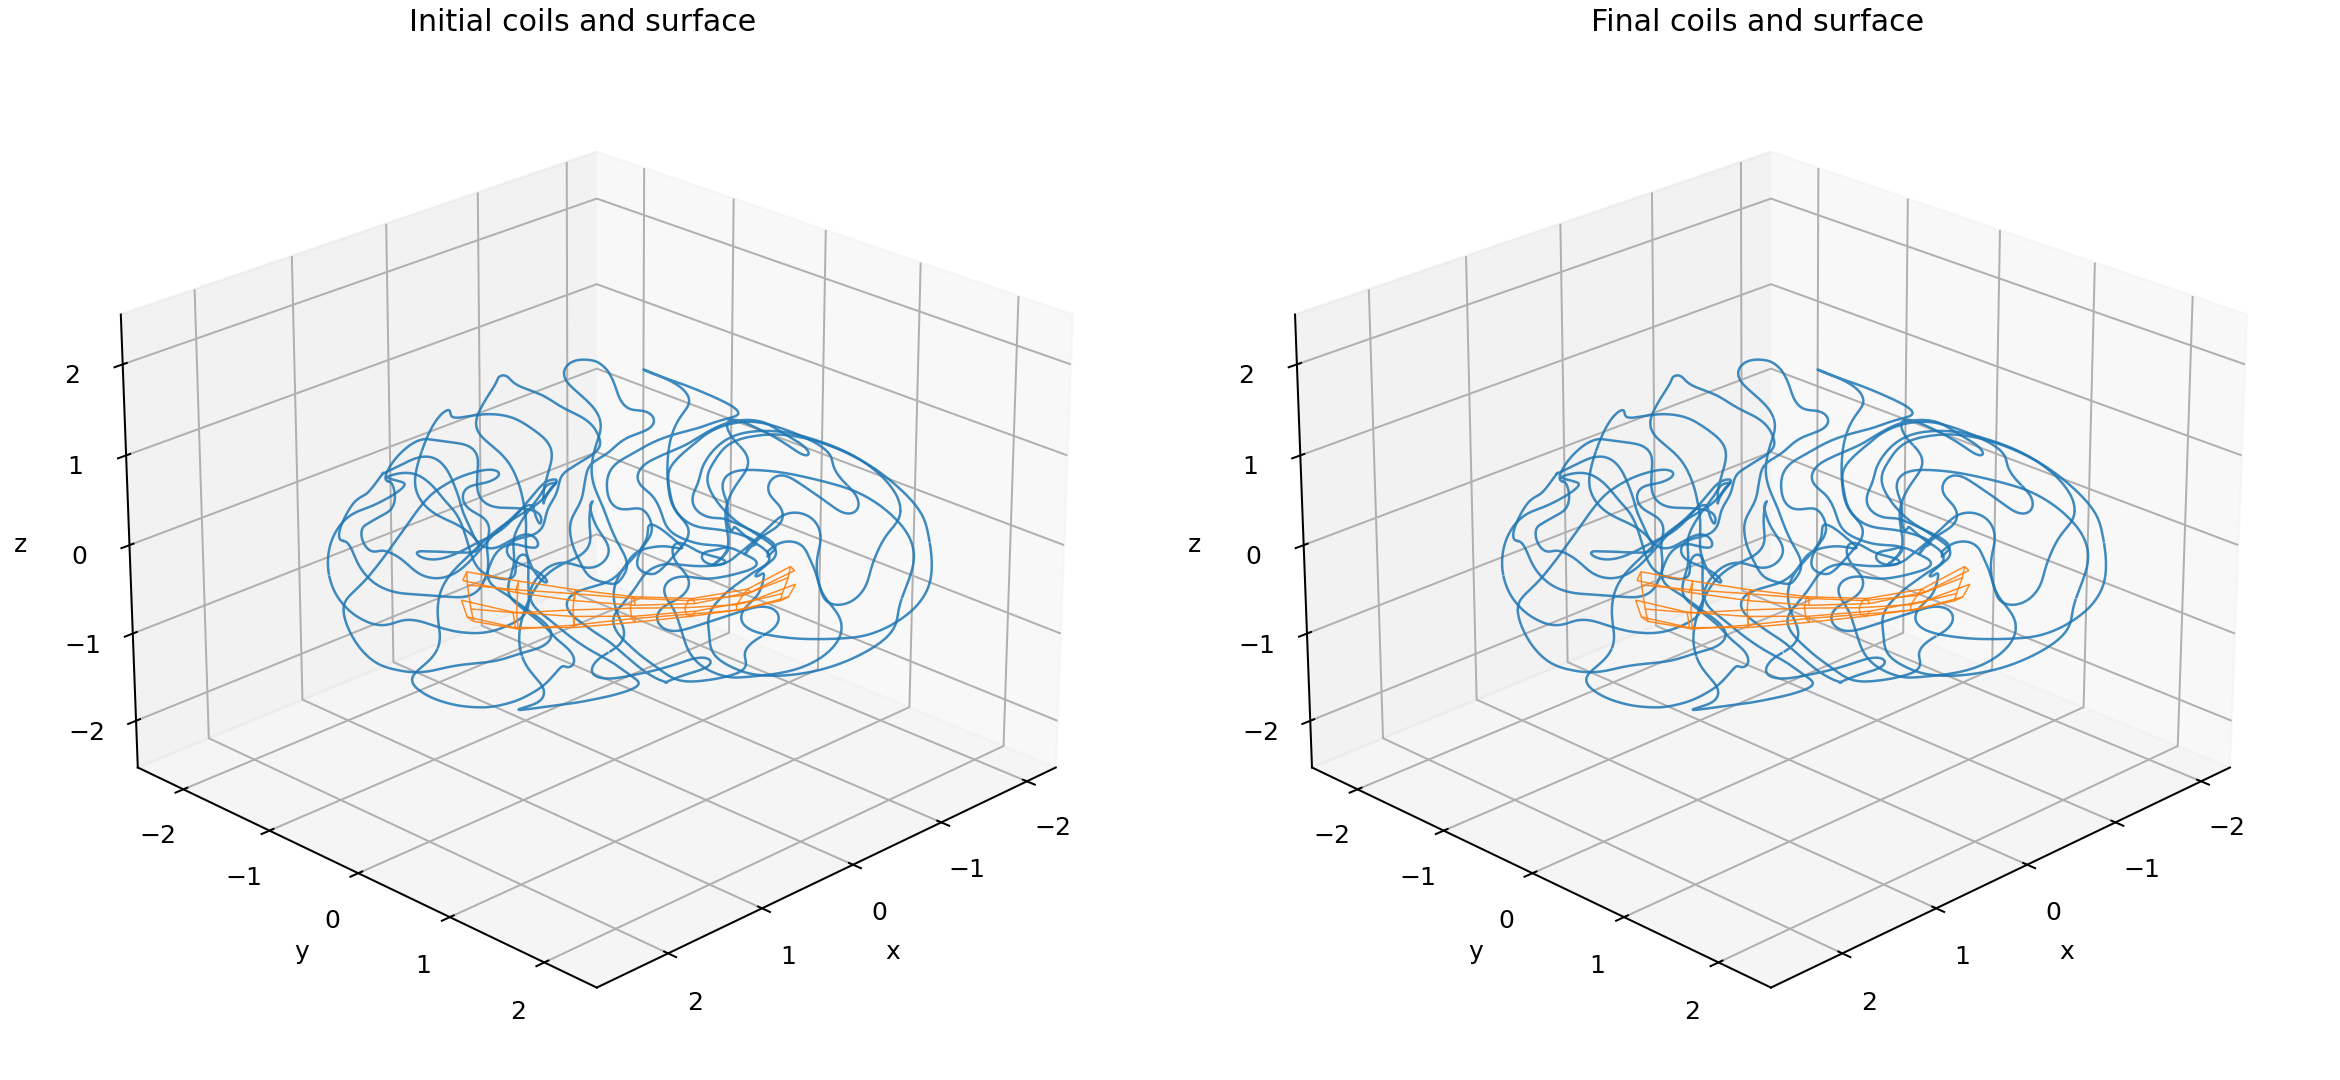
\includegraphics[width=0.97\linewidth]{output/boozerQA_finitebeta_geometry_comparison.png}
\caption{Initial and final coil-plus-surface geometry from the generated VTK outputs. The left panel uses the initial seed configuration, while the right panel shows the configuration after the finite-beta workflow.}
\label{fig:geometry}
\end{figure}

\subsection{State maps on the optimized surface}
Figure \ref{fig:statecompare} shows two key finite-beta surface diagnostics. The top row plots the quasi-axisymmetric defect measured as $|\mathbf{B}| - \langle |\mathbf{B}| \rangle_{\phi}$ at fixed poloidal index, which is the same weighted quantity used by the non-quasisymmetric ratio diagnostic. The bottom row plots the magnetic pressure-jump residual. The optimized state drives the pressure-jump map to numerical zero on the displayed scale, which is exactly what the inner finite-beta closure is meant to enforce.

\begin{figure}[H]
\centering
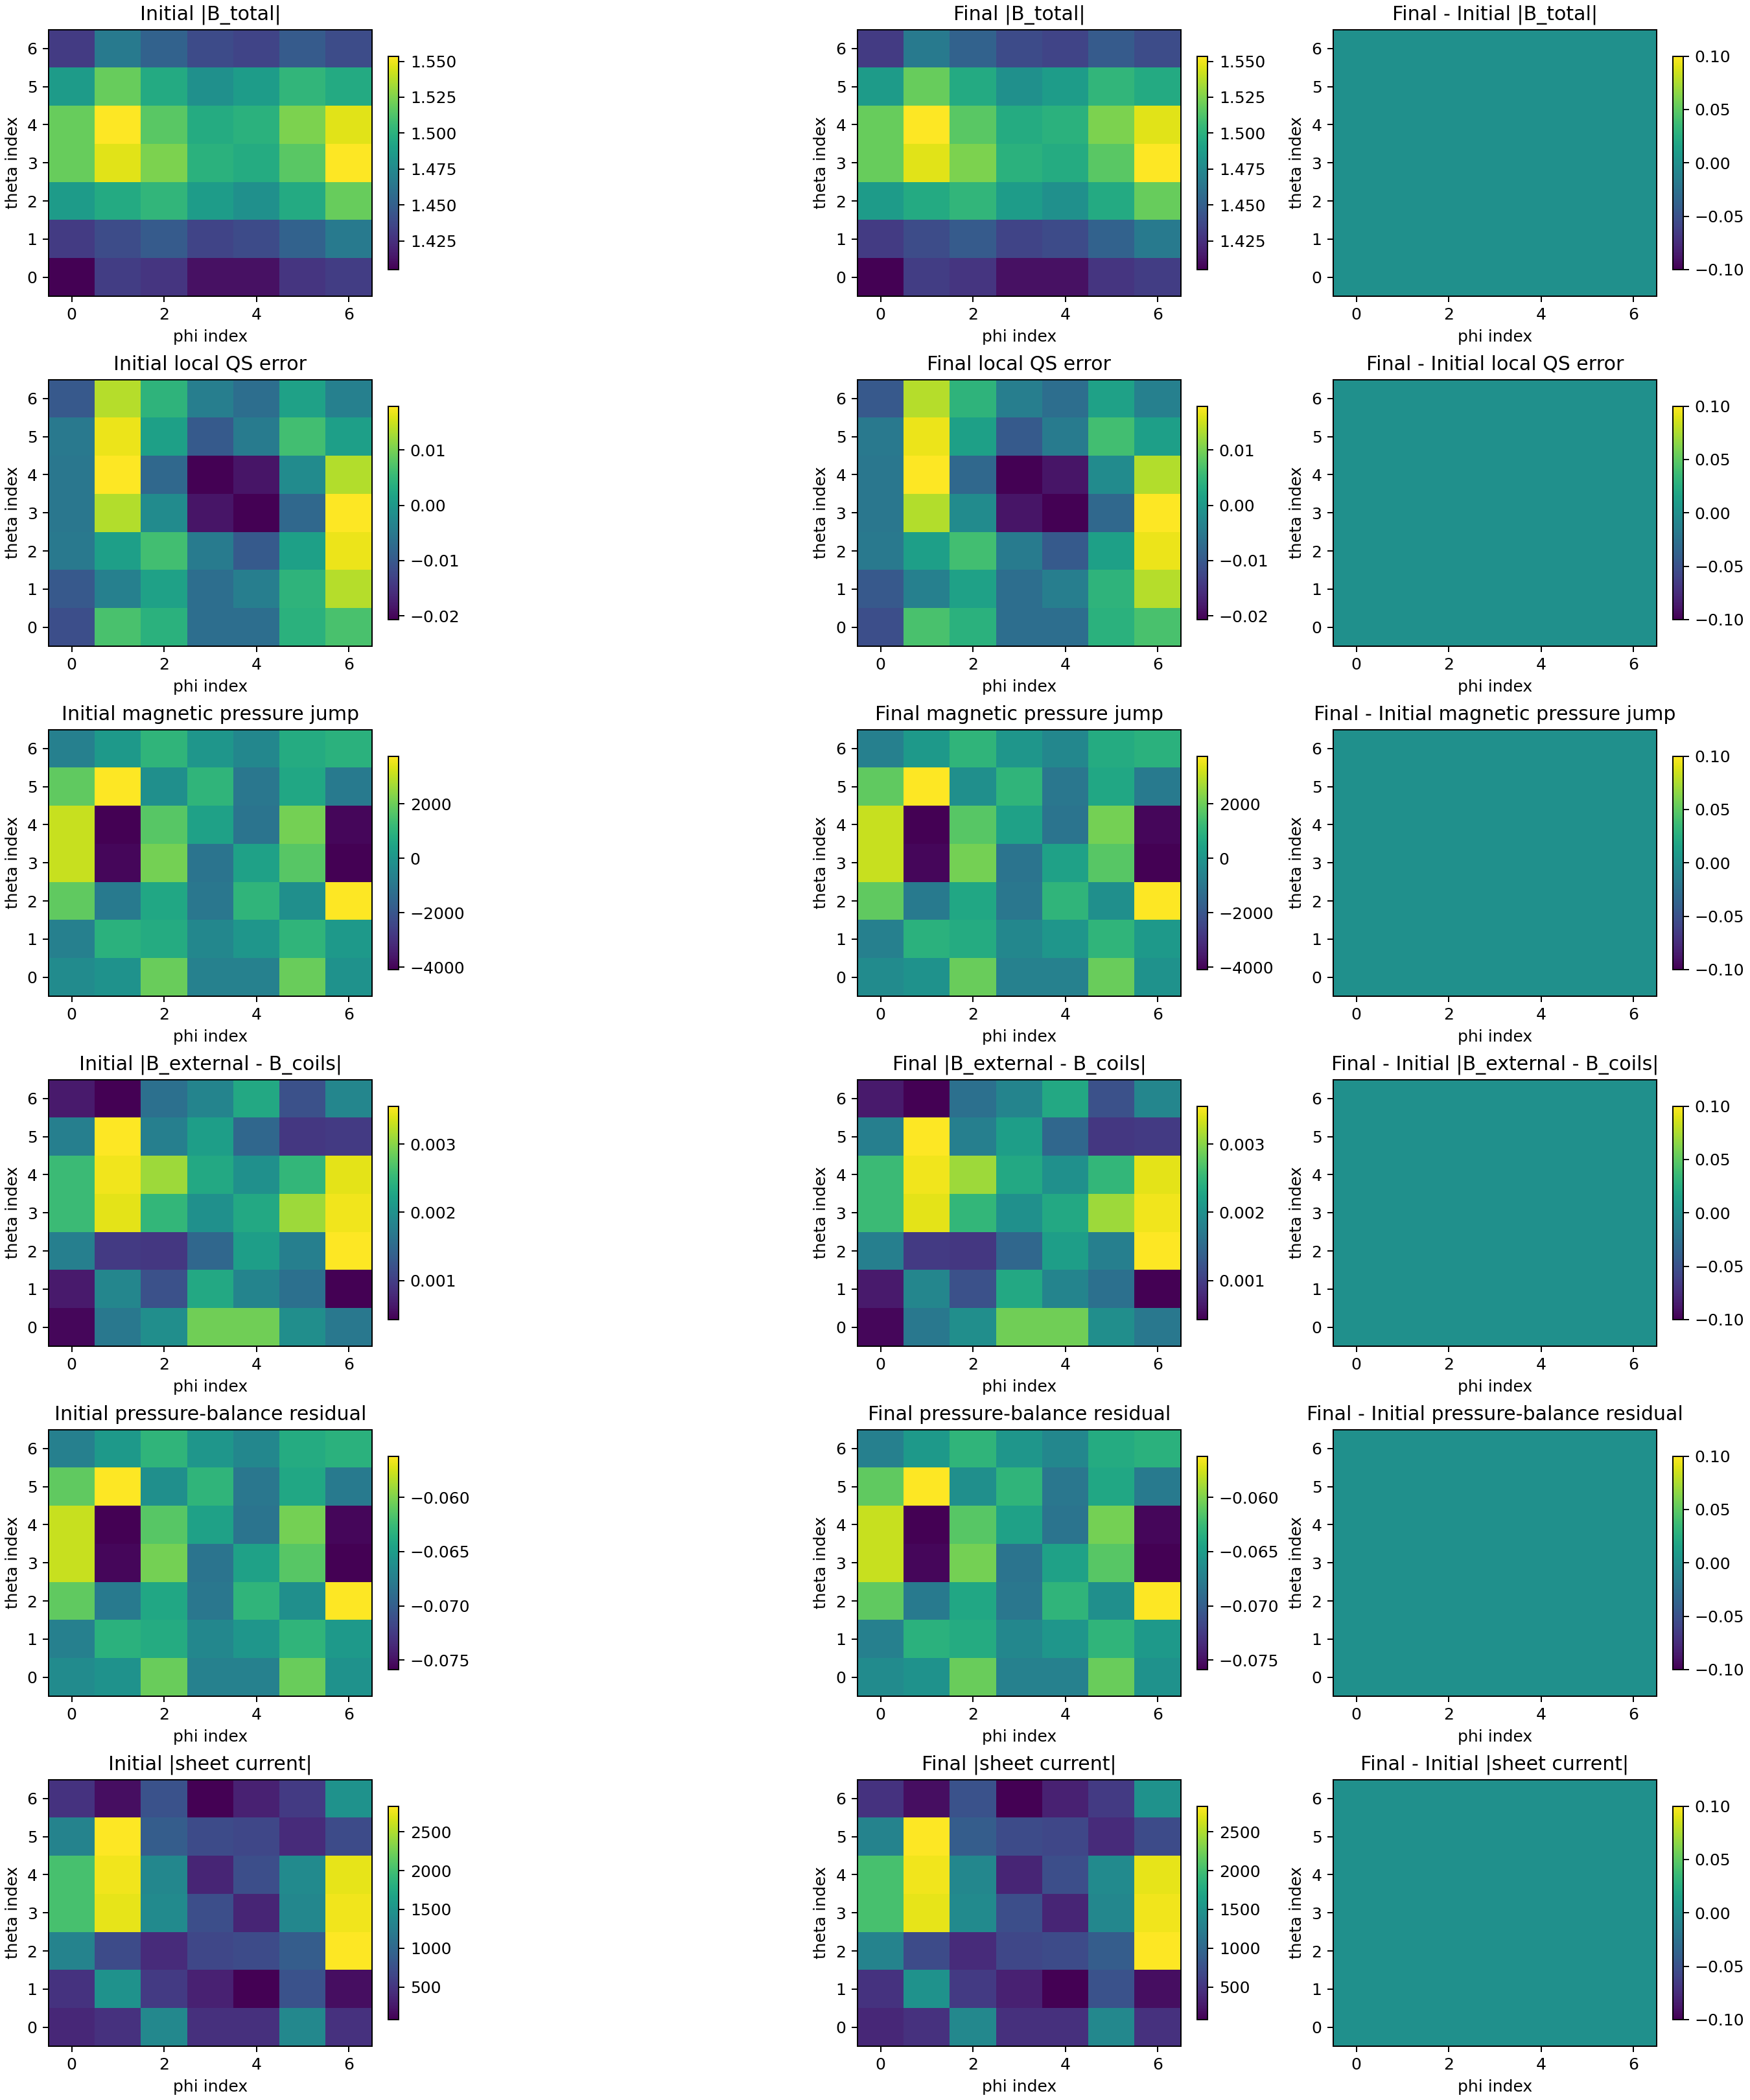
\includegraphics[width=0.98\linewidth]{output/boozerQA_finitebeta_state_comparison.png}
\caption{State comparison from the current run artifacts. Top: quasi-axisymmetric defect maps. Bottom: magnetic pressure-jump maps. The final pressure-jump map is visually flat because the finite-beta inner solve has reduced that residual to the numerical noise floor on this grid.}
\label{fig:statecompare}
\end{figure}

\subsection{Objective trade-offs before and after the inner closure}
Figure \ref{fig:objectivecompare} and Table \ref{tab:metrics} summarize the most important scalar diagnostics extracted from the boundary VTK files. Two features are worth highlighting.

\begin{enumerate}
\item The finite-beta inner closure greatly reduces the normal and pressure blocks, driving them from $\mathcal{O}(10^{-3})$ and $\mathcal{O}(10^{-3})$ down to $\mathcal{O}(10^{-7})$ and $\mathcal{O}(10^{-9})$, respectively.
\item The coil-match block grows, which is physically and numerically plausible: once pressure balance is enforced self-consistently, the surface is no longer the vacuum surface, so the finite-beta closure trades some coil-match error to satisfy the jump conditions and tangency more accurately.
\end{enumerate}

\begin{figure}[H]
\centering
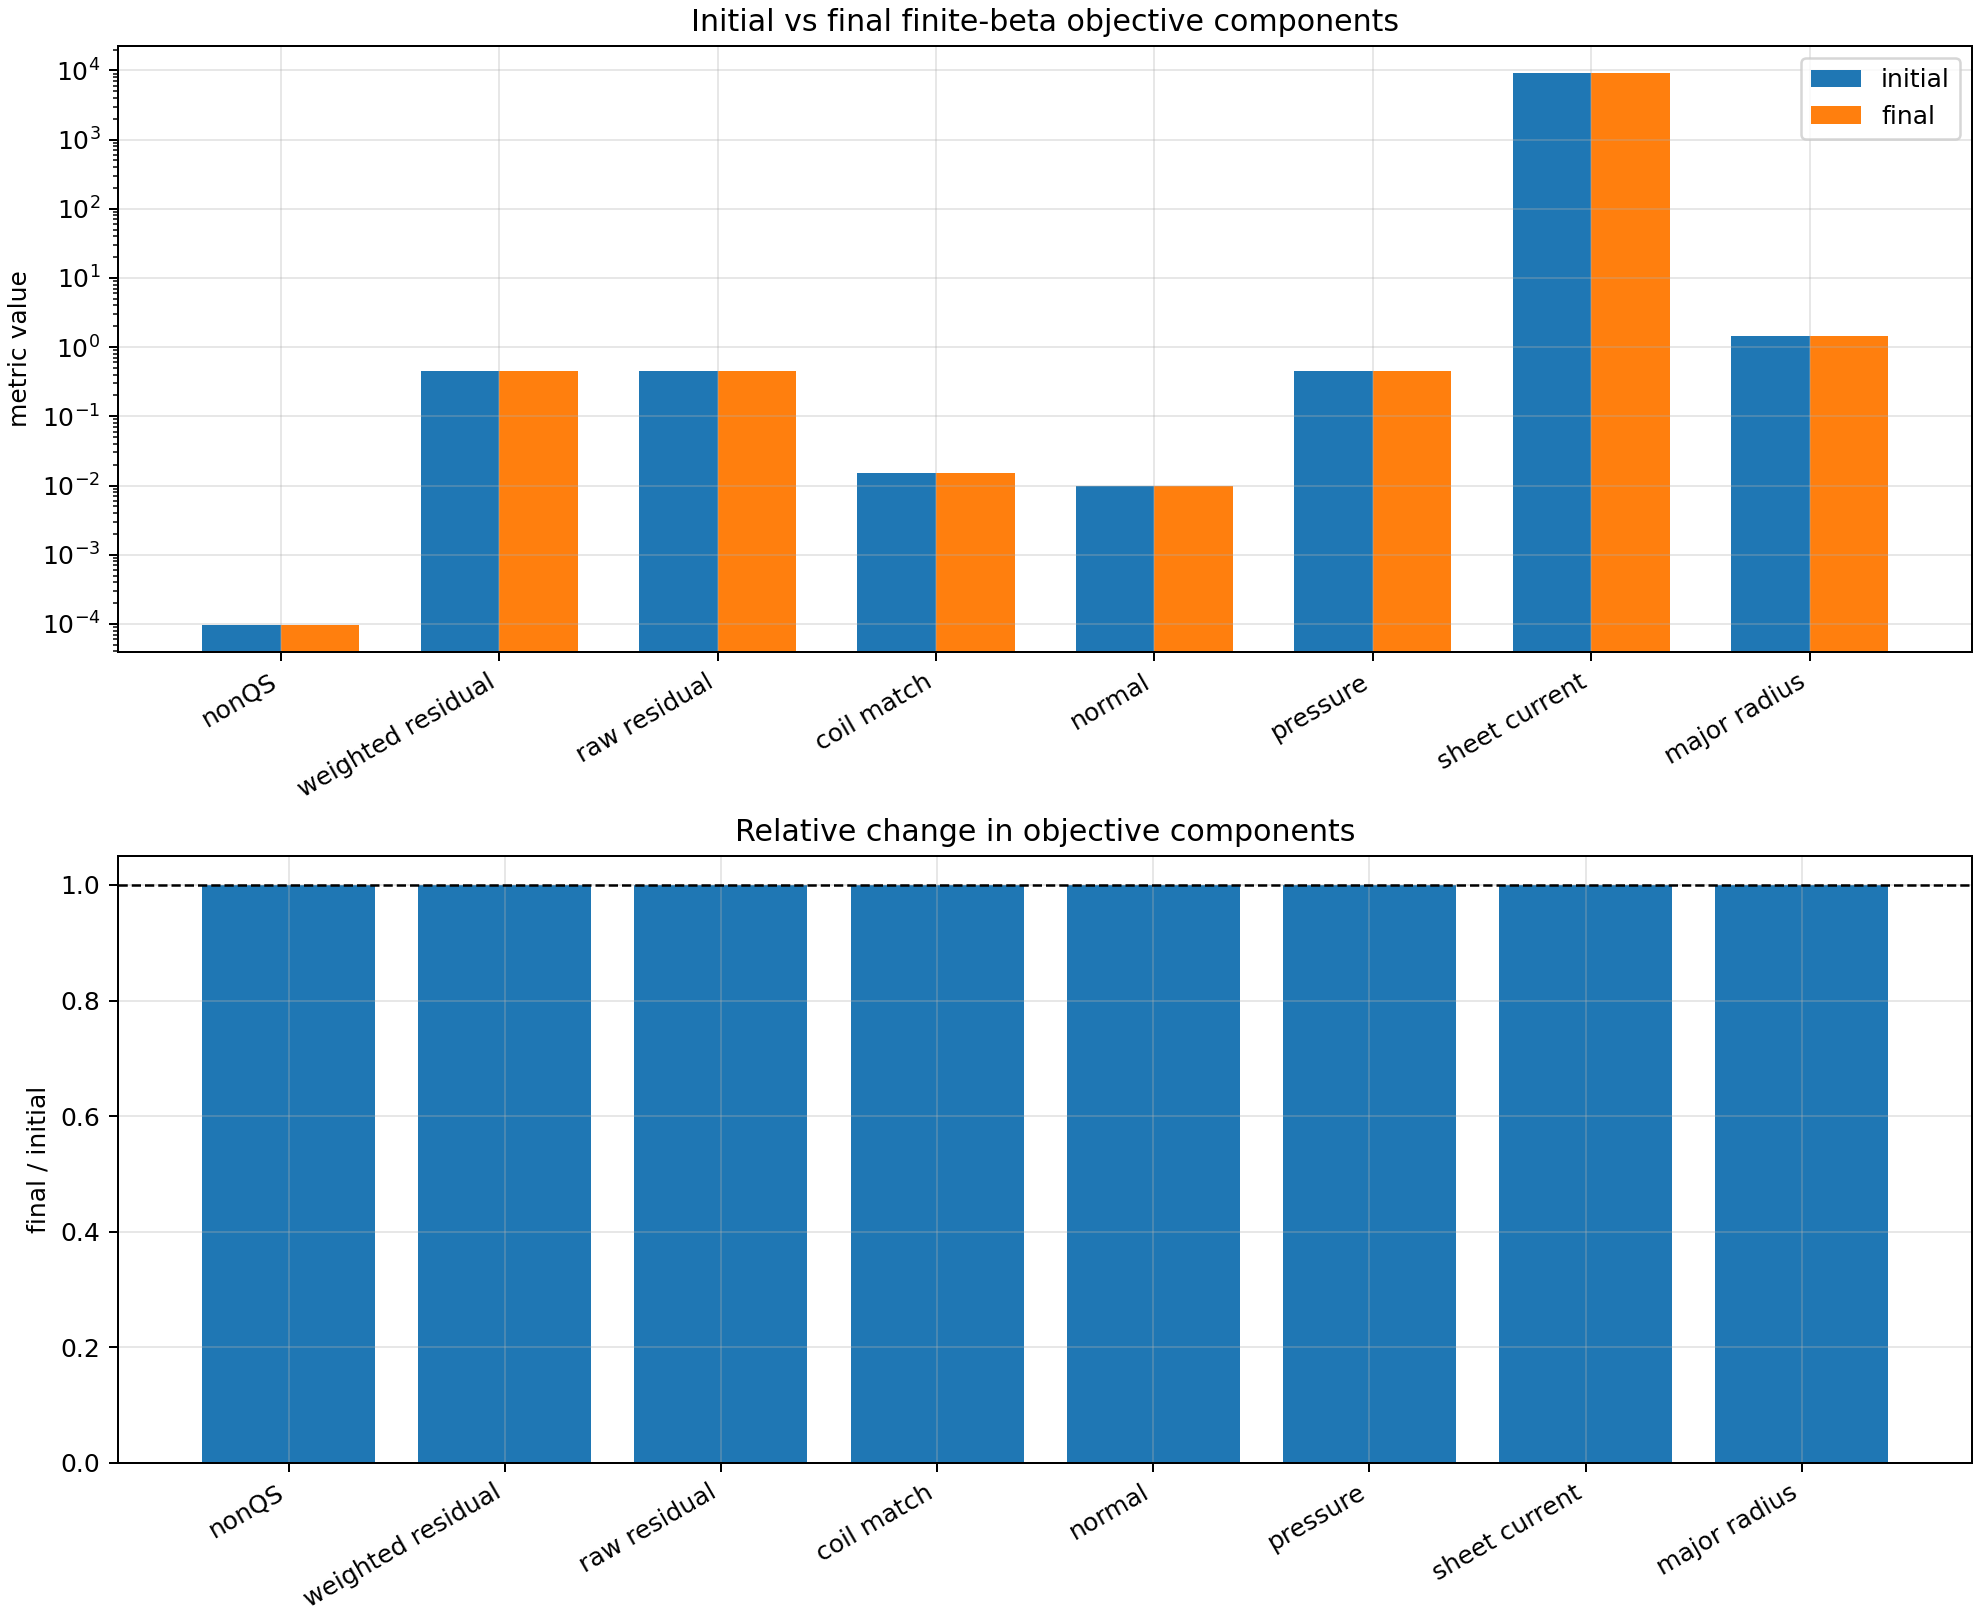
\includegraphics[width=0.98\linewidth]{output/boozerQA_finitebeta_objective_comparison.png}
\caption{Before-and-after scalar comparison derived from the VTK output. The left panel focuses on residual and quasisymmetry measures. The right panel shows state and diagnostic quantities on a logarithmic scale so that the surface radius and field-strength levels remain visible next to the much larger sheet-current diagnostic.}
\label{fig:objectivecompare}
\end{figure}

\begin{table}[H]
\centering
\caption{Current initial and final scalar diagnostics extracted from \texttt{boozerQA\_finitebeta\_boundary\_init.vts} and \texttt{boozerQA\_finitebeta\_boundary.vts}.}
\label{tab:metrics}
\begin{tabular}{lrr}
\toprule
Metric & Initial & Final \\
\midrule
QA ratio & $8.5299 \times 10^{-4}$ & $7.9279 \times 10^{-4}$ \\
Coil-match RMS & $2.1906 \times 10^{-3}$ & $5.5065 \times 10^{-3}$ \\
Normal RMS & $1.3200 \times 10^{-3}$ & $4.5992 \times 10^{-7}$ \\
Pressure RMS & $4.9211 \times 10^{-3}$ & $7.1966 \times 10^{-9}$ \\
Mean $|\mathbf{K}|$ & $1.1043 \times 10^{3}$ & $6.4590 \times 10^{2}$ \\
Mean $R$ & $1.4868604$ & $1.4868485$ \\
Mean $|\mathbf{B}_{\mathrm{total}}|$ & $1.4782175$ & $1.4781828$ \\
Mean $|\mathbf{B}_{\mathrm{external}}|$ & $1.4782805$ & $1.4781828$ \\
\bottomrule
\end{tabular}
\end{table}

\subsection{Frozen-state direct versus full virtual casing}
The most important follow-on diagnostic after the principal-value direct closure update is to remove geometry drift from the comparison and evaluate the direct closure and the full virtual-casing operator on the same frozen state. The code now writes those comparisons to \texttt{output/direct\_closure\_compare}, both at the vacuum seed and at the final reduced direct state.

Figure \ref{fig:directvcfrozen} shows the final frozen-state comparison. The direct and VC exterior fields are visibly close at the map level, but the associated coil-match, normal, and pressure blocks remain meaningfully different. This is exactly the distinction that matters physically: improving the local exterior field approximation can reduce the raw field mismatch without yet reproducing the same finite-beta response once the jump and pressure equations are re-evaluated.

\begin{figure}[H]
\centering

\includegraphics[width=0.98\linewidth]{output/direct_closure_compare/boozerQA_finitebeta_direct_vs_vc_final.png}
\caption{Frozen-state comparison between the direct principal-value closure and the full virtual-casing closure on the same final reduced direct state. The first two columns compare the direct and VC maps directly, while the third column shows the pointwise difference.}
\label{fig:directvcfrozen}
\end{figure}

Table \ref{tab:directvcfrozen} summarizes the key numbers from those frozen-state diagnostics. Two facts stand out. First, the exterior field itself is already rather close: the relative difference is $1.47 \times 10^{-3}$ at the vacuum seed and $4.61 \times 10^{-3}$ at the final reduced direct state. Second, that modest field mismatch still translates into much larger differences in the pressure and sheet-current diagnostics after the closure equations are replayed. This is strong evidence that the remaining direct-versus-VC discrepancy is not just an offset-surface artifact; it is tied to the way the closure responds globally to the field on the surface.

\begin{table}[H]
\centering
\caption{Frozen-state direct-versus-VC comparison from the reduced direct branch. The ``initial'' row is the vacuum seed state and the ``final'' row is the reduced $1\%$ beta direct state.}
\label{tab:directvcfrozen}
\begin{tabular}{lrrrrrr}
\toprule
State & $\|\Delta B_{\mathrm{ext}}\|/\|B_{\mathrm{ext}}^{\mathrm{VC}}\|$ & $\|r_{\mathrm{jump}}^{\mathrm{dir}}\|$ & $\|r_p^{\mathrm{dir}}\|$ & $\|r_p^{\mathrm{VC}}\|$ & $\|K^{\mathrm{dir}}\|$ & $\|K^{\mathrm{VC}}\|$ \\
\midrule
Initial & $1.4666 \times 10^{-3}$ & $6.1731 \times 10^{-15}$ & $1.5289 \times 10^{-14}$ & $3.1478 \times 10^{-2}$ & $4.9124 \times 10^{-9}$ & $9.1304 \times 10^{3}$ \\
Final & $4.6139 \times 10^{-3}$ & $4.6478 \times 10^{-2}$ & $1.7303 \times 10^{-2}$ & $1.5187 \times 10^{-1}$ & $3.7103 \times 10^{4}$ & $9.0933 \times 10^{3}$ \\
\bottomrule
\end{tabular}
\end{table}

\subsection{Reduced branch comparison with VC and VMEC}
The frozen-state diagnostic isolates the closure error on one fixed state. A complementary question is how the reduced direct, VC, and VMEC-backed branches compare at the level of their final reduced solves. Table \ref{tab:branchcompare} records that comparison using the reduced benchmark note in \texttt{docs/source/finite\_beta\_direct\_closure\_note.md}.

The key comparison is direct versus the single-surface VC surrogate. On the reduced $1\%$ beta QA benchmark, the two branches stay reasonably close in $\iota$ but differ strongly in the inferred finite-beta current response: the direct branch ends at $I \approx 1.54 \times 10^{-1}$, while the VC branch ends at $I \approx 5.01 \times 10^{-3}$. The VMEC-backed branch still serves mainly as a wiring stress test in this report because the available interface fields imply an effective beta of about $100\%$, so it is not an apples-to-apples validator for the reduced $1\%$ direct and VC cases.

\begin{table}[H]
\centering
\caption{Reduced finite-beta branch comparison. The direct and VC rows correspond to the reduced $1\%$ beta QA benchmark in the direct-closure note. The VMEC-backed row is included as a branch-wiring stress test, not as a matched validator for the $1\%$ case.}
\label{tab:branchcompare}
\begin{tabular}{lrrrrl}
\toprule
Branch & $\iota$ & $G$ & $I$ & Residual norm & Comment \\
\midrule
Direct self-consistent & $-4.064341 \times 10^{-1}$ & $1.388384 \times 10^{1}$ & $1.535492 \times 10^{-1}$ & $4.960470 \times 10^{-2}$ & principal-value direct closure \\
Single-surface VC & $-3.951105 \times 10^{-1}$ & $1.388384 \times 10^{1}$ & $5.012459 \times 10^{-3}$ & weighted $7.705521 \times 10^{-2}$, raw $1.656266 \times 10^{-1}$ & VC surrogate \\
VMEC-backed & $2.084661 \times 10^{-1}$ & $0$ & $-7.223725 \times 10^{-1}$ & $1.895913 \times 10^{1}$ & inferred $\beta \approx 100\%$ \\
\bottomrule
\end{tabular}
\end{table}

\subsection{Outer optimization and pressure continuation evidence}
The original example already produced two important optimization-level summaries, which remain useful in the revised workflow.

\begin{figure}[H]
\centering
\begin{subfigure}[t]{0.48\linewidth}
\centering
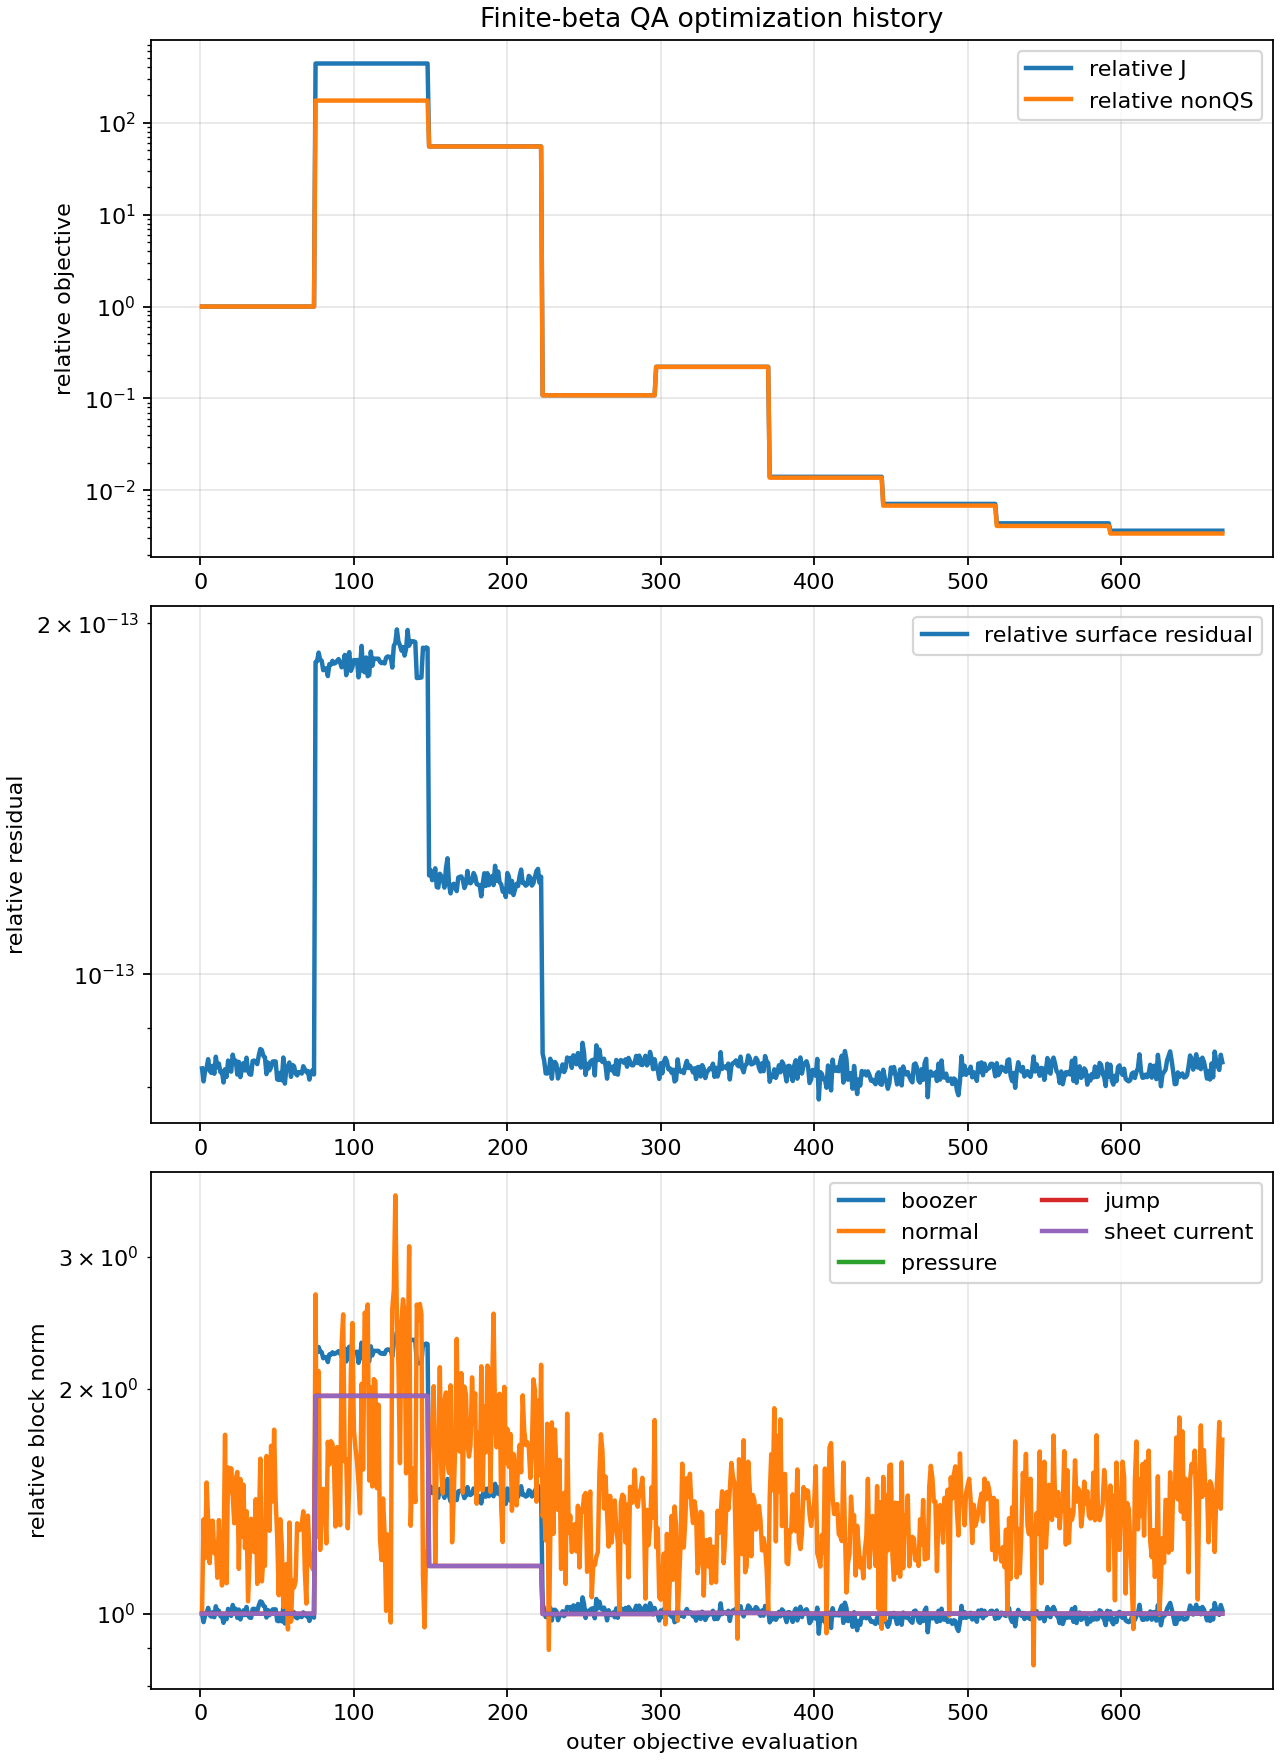
\includegraphics[width=\linewidth]{output/boozerQA_finitebeta_history.png}
\caption{Outer reduced QA history.}
\end{subfigure}
\hfill
\begin{subfigure}[t]{0.48\linewidth}
\centering
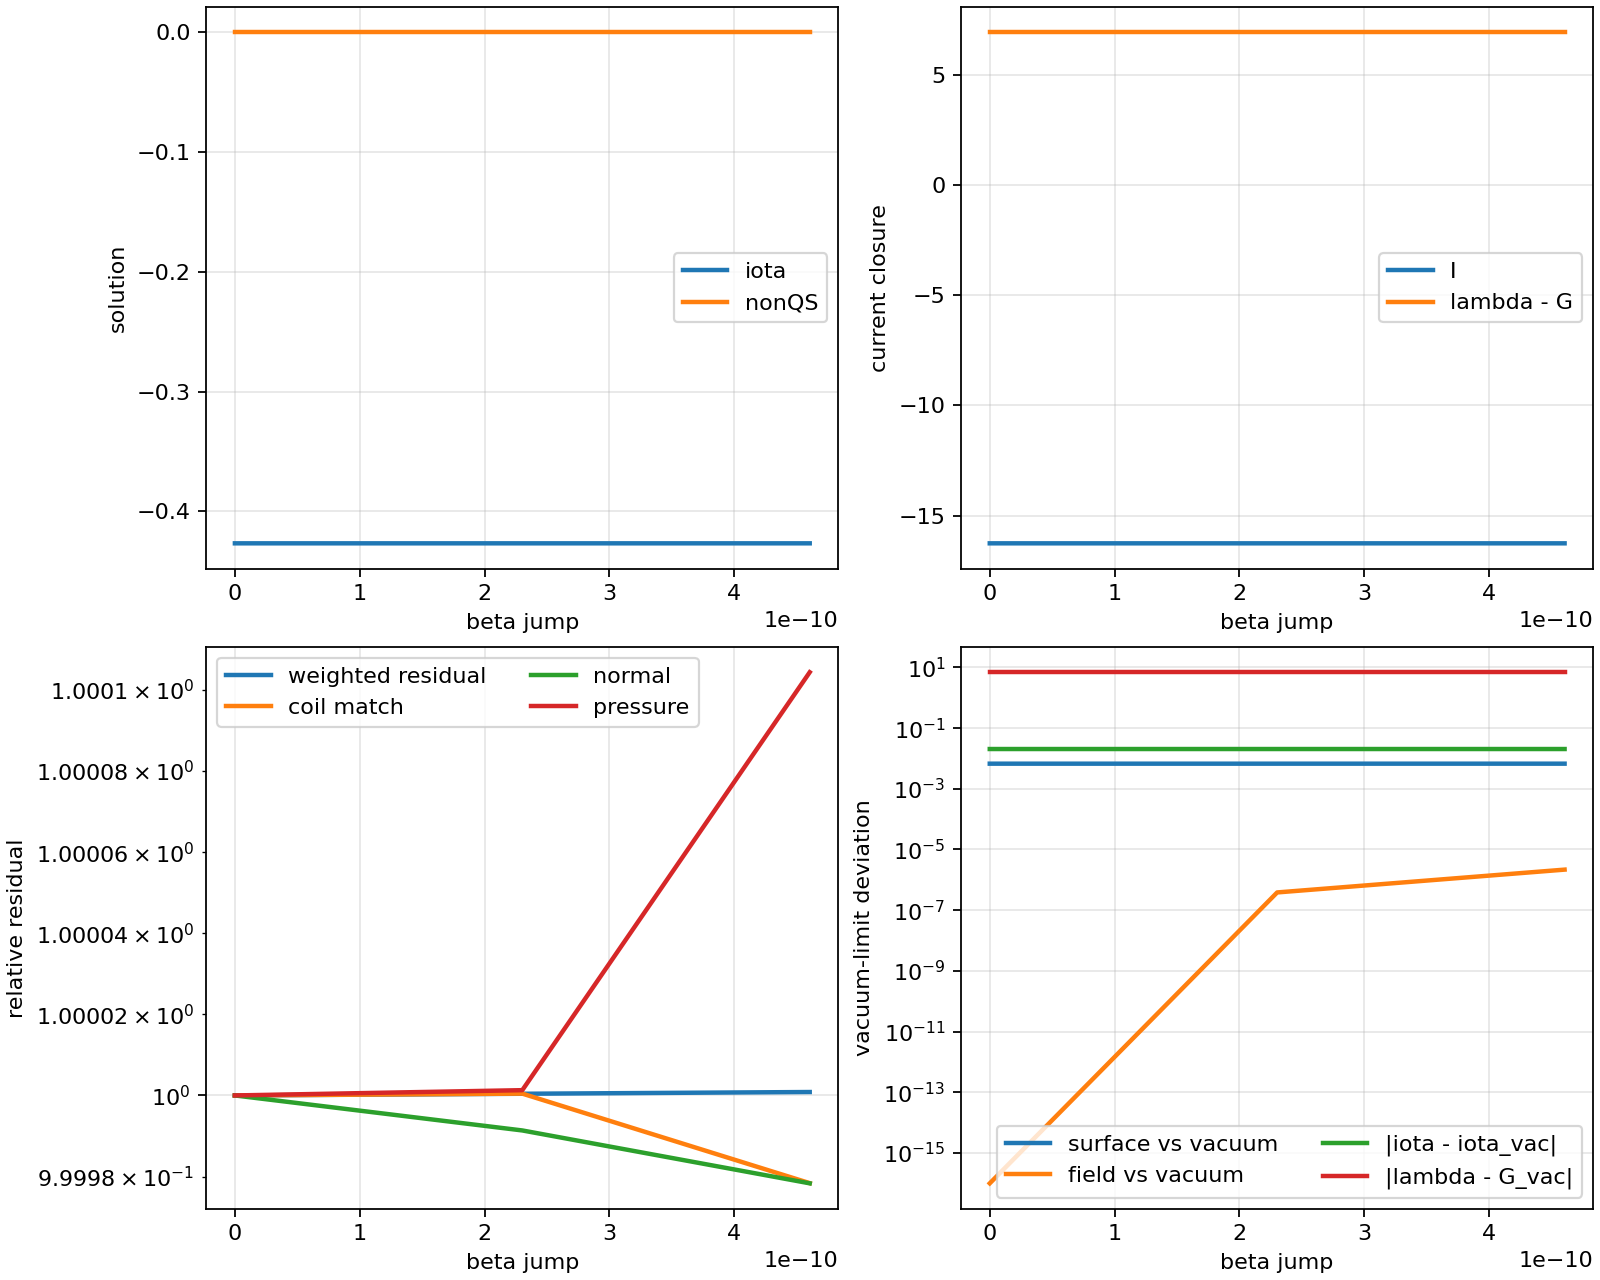
\includegraphics[width=\linewidth]{output/boozerQA_finitebeta_pressure_scan.png}
\caption{Pressure scan from the vacuum limit to the target jump.}
\end{subfigure}
\caption{Optimization-level diagnostics written directly by the example workflow. The outer loop history shows the reduced QA search, while the pressure scan reports how the single-surface finite-beta state departs from the vacuum reference as the pressure jump is increased.}
\label{fig:historypressure}
\end{figure}

The current artifact summary reports the following run-level statistics:

\begin{itemize}
\item Outer reduced QA history: $666$ evaluations, initial objective $J = 3.6385 \times 10^{-3}$, best objective $J = 1.3259 \times 10^{-5}$, best major radius $R_0 = 1.47007$, and best $\iota = -0.31$.
\item Pressure scan: three samples from the vacuum limit to $\Delta p = 4.0 \times 10^{-4}$, corresponding to a reported final $\beta$ jump of $4.6057 \times 10^{-10}$, final $\iota = -0.4267719783556057$, final $\Lambda = 13.88411653352608$, and final non-quasisymmetric ratio $8.6263 \times 10^{-5}$.
\end{itemize}

These numbers are not yet a final physics-validation benchmark. They are evidence that the finite-beta closure, reduced outer loop, and pressure continuation pipeline are all numerically connected and producing coherent artifacts.

\section{Comparison with Existing Literature}
\subsection{Relative to direct Boozer optimization in vacuum}
The methods of Giuliani et al. \cite{Giuliani2022,Giuliani2023} solve a direct surface problem in vacuum. Their essential strength is that the surface itself becomes the optimization variable and the Boozer constraints are enforced without introducing a separate equilibrium solver in the loop. The present work preserves exactly that spirit.

The key extension beyond the vacuum literature is that the field is no longer treated as known from the coils alone. Instead, the total field is parameterized on the surface, the exterior field is reconstructed from virtual casing, and magnetic pressure balance is enforced on the same surface. In that sense, this branch extends the \emph{direct surface formulation} to finite beta.

\subsection{Relative to finite-beta optimization based on full equilibria}
Finite-beta stellarator optimization in the literature commonly relies on full equilibrium models, for good reason \cite{Baillod2022,HirshmanWhitson1983}. Those models incorporate global force balance, topology, and consistency across the plasma volume. The method described here does not replace them.

What this branch contributes instead is an intermediate model between vacuum direct Boozer optimization and full finite-beta equilibrium optimization:

\begin{itemize}
\item richer than vacuum because it enforces a nonzero pressure jump and the associated magnetic stress balance;
\item cheaper than full equilibrium because it closes only on one surface;
\item directly usable inside \texttt{simsopt}'s optimization infrastructure because it preserves a surface-residual least-squares structure.
\end{itemize}

That is the correct scientific framing. The method goes beyond the existing direct-Boozer vacuum literature by incorporating finite-beta surface closure, but it does not supersede volume-equilibrium methods for final validation.

\subsection{Relative to prior staged formulations in this branch}
Earlier stages of this project used prescribed internal and external fields as a manufactured finite-beta stepping stone. That work remains useful for derivative checks and controlled tests, but the present branch now has a stronger central story: the field split is self-consistently constructed from the current surface itself. This is the point at which the implementation becomes scientifically aligned with the original no-VMEC objective.

\section{Limitations and Honest Scope}
The current implementation has four important limitations.

\begin{enumerate}
\item It is a single-surface closure, not a full nested-volume equilibrium. A small residual on one surface does not by itself guarantee a globally acceptable finite-beta equilibrium.
\item The free-surface Jacobian is only partially exact. The scalar derivatives with respect to $\iota$ and $\Lambda$ are exact for fixed geometry, but the VC source-surface shape derivative is not available in the current compiled library, so the geometry block is approximated by structured finite differences.
\item The outer coil optimization is reduced-dimensional for practicality. The method is not yet a drop-in replacement for the full vacuum \texttt{boozerQA.py} optimization campaign.
\item Environment-specific import friction remains present in the local checkout, notably through the compiled \texttt{vmec} import path. Report-generation post-processing was therefore separated into a lightweight script that reads the generated VTK and CSV artifacts directly.
\end{enumerate}

None of these limitations invalidate the method. They define the current maturity level and the next engineering targets.

\section{Recommended Next Steps}
The natural follow-on tasks are now well defined.

\begin{enumerate}
\item Expose or derive exact source-surface derivatives of the virtual-casing operator so the free-surface Jacobian can become fully analytic.
\item Promote the reduced outer coil optimization to the same breadth of coil degrees of freedom used in the vacuum workflow once the inner Jacobian and runtime are strong enough.
\item Validate the single-surface finite-beta solutions against full finite-beta equilibria from VMEC or related free-boundary calculations across a family of pressure and current profiles.
\item Extend the diagnostics from one-surface agreement to multi-surface or volume-consistency probes so the gap between this closure model and a global equilibrium can be quantified directly.
\end{enumerate}

\section{Conclusion}
The finite-beta Boozer-surface work in this checkout now has a coherent mathematical and software identity. The code no longer depends on a staged prescribed-field narrative to explain finite-beta behavior. Instead, it implements a direct self-consistent closure on one surface:
\begin{equation}
  (\mathbf{x},\iota,\Lambda)
  \longrightarrow
  \mathbf{B}_{\mathrm{total}}
  \longrightarrow
  \mathcal{V}[\mathbf{x},\mathbf{B}_{\mathrm{total}}]
  \longrightarrow
  \{\mathbf{r}_{\mathrm{coil}}, r_{\mathrm{normal}}, r_{\mathrm{pressure}}\}.
\end{equation}

This is the precise sense in which the branch now supports finite-beta Boozer optimization without embedding VMEC in the inner loop. The implementation is deliberately surgical, preserves compatibility with the vacuum code, introduces exact scalar derivatives where available, and adds the diagnostic infrastructure needed to study the new model quantitatively. The new frozen-state benchmark sharpens the technical conclusion: the principal-value direct closure gets the exterior field surprisingly close to the full virtual-casing result, but the replayed pressure and sheet-current blocks still differ enough to explain the remaining direct-versus-VC current mismatch. The present method is best viewed as a practical finite-beta optimization closure for direct Boozer workflows. It goes beyond the vacuum literature in exactly that direction, while remaining honest about the need for future global-equilibrium validation.

\begin{thebibliography}{99}

\bibitem{Boozer1981}
A. H. Boozer, ``Plasma equilibrium with rational magnetic surfaces,'' \emph{Physics of Fluids}, vol. 24, no. 11, pp. 1999--2003, 1981. doi: \href{https://doi.org/10.1063/1.863297}{10.1063/1.863297}.

\bibitem{HirshmanWhitson1983}
S. P. Hirshman and J. C. Whitson, ``Steepest-descent moment method for three-dimensional magnetohydrodynamic equilibria,'' \emph{Physics of Fluids}, vol. 26, no. 12, pp. 3553--3568, 1983. doi: \href{https://doi.org/10.1063/1.864116}{10.1063/1.864116}.

\bibitem{Giuliani2022}
A. Giuliani, F. Wechsung, G. Stadler, A. Cerfon, and M. Landreman, ``Direct computation of magnetic surfaces in Boozer coordinates and coil optimization for quasisymmetry,'' \emph{Journal of Plasma Physics}, vol. 88, no. 4, 905880401, 2022. doi: \href{https://doi.org/10.1017/S0022377822000563}{10.1017/S0022377822000563}.

\bibitem{Giuliani2023}
A. Giuliani, F. Wechsung, A. Cerfon, M. Landreman, and G. Stadler, ``Direct stellarator coil optimization for nested magnetic surfaces with precise quasi-symmetry,'' \emph{Physics of Plasmas}, vol. 30, no. 4, 042511, 2023. doi: \href{https://doi.org/10.1063/5.0129716}{10.1063/5.0129716}.

\bibitem{Baillod2022}
A. Baillod, J. Loizu, J. P. Graves, and M. Landreman, ``Stellarator optimization for nested magnetic surfaces at finite $\beta$ and toroidal current,'' \emph{Physics of Plasmas}, vol. 29, no. 4, 042505, 2022. doi: \href{https://doi.org/10.1063/5.0080809}{10.1063/5.0080809}.

\bibitem{Landreman2021}
M. Landreman \emph{et al.}, ``SIMSOPT: A flexible framework for stellarator optimization,'' \emph{Journal of Open Source Software}, vol. 6, no. 65, 3525, 2021. doi: \href{https://doi.org/10.21105/joss.03525}{10.21105/joss.03525}.

\bibitem{Wechsung2022}
F. Wechsung, M. Landreman, A. Giuliani, A. Cerfon, and G. Stadler, ``Precise stellarator quasi-symmetry can be achieved with electromagnetic coils,'' \emph{Proceedings of the National Academy of Sciences}, vol. 119, no. 13, e2202084119, 2022. doi: \href{https://doi.org/10.1073/pnas.2202084119}{10.1073/pnas.2202084119}.

\bibitem{Malhotra2020}
D. Malhotra, A. J. Cerfon, M. O'Neil, and E. Toler, ``Efficient high-order singular quadrature schemes in magnetic fusion,'' \emph{Plasma Physics and Controlled Fusion}, vol. 62, 024004, 2020. doi: \href{https://doi.org/10.1088/1361-6587/ab4a7f}{10.1088/1361-6587/ab4a7f}.

\end{thebibliography}

\end{document}